\section{Disentanglement restricted inside spherical regions of \textit{k}-space LaVO$_3$.}
\label{sec20:LaVO3}

\begin{itemize}
	\item Outline: {\it Obtain disentangled MLWFs for strained $\mathrm{LaVO}_3$.}
\end{itemize}

\begin{figure}[h!]
\centering
\subfloat[LaVO$_3$]{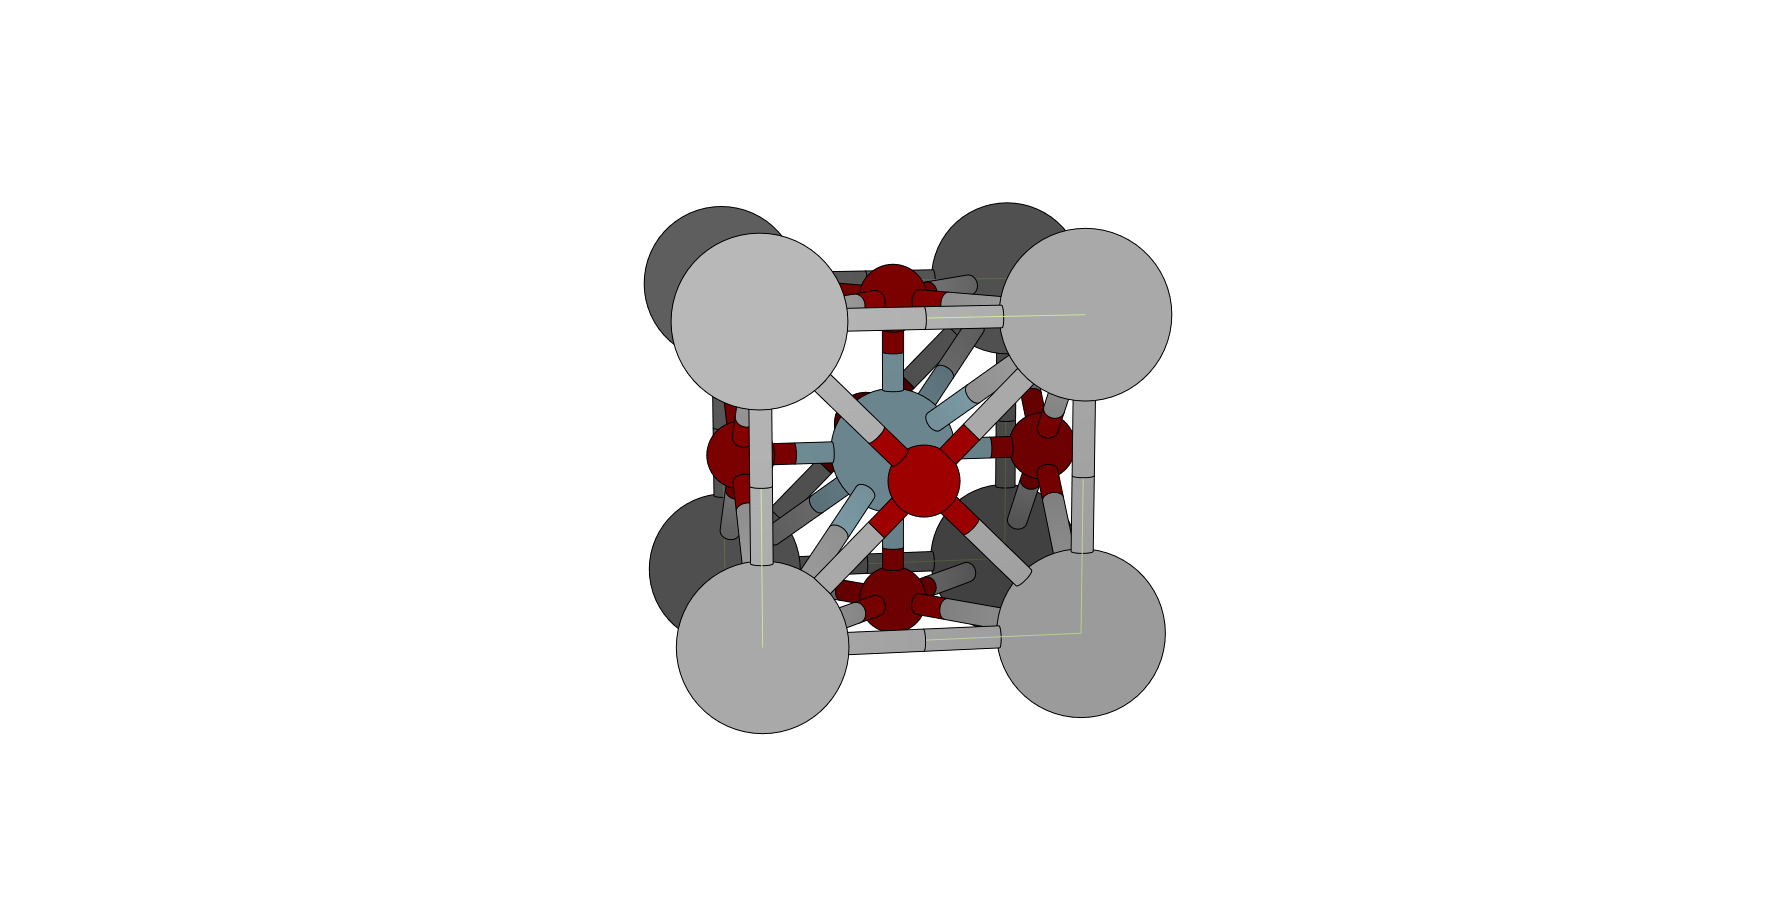
\includegraphics[width=0.45\columnwidth,trim={300pt 10pt 300pt 150pt},clip]{figure/example20/LaVO3.png}}
\centering
\subfloat[SrMnO$_3$]{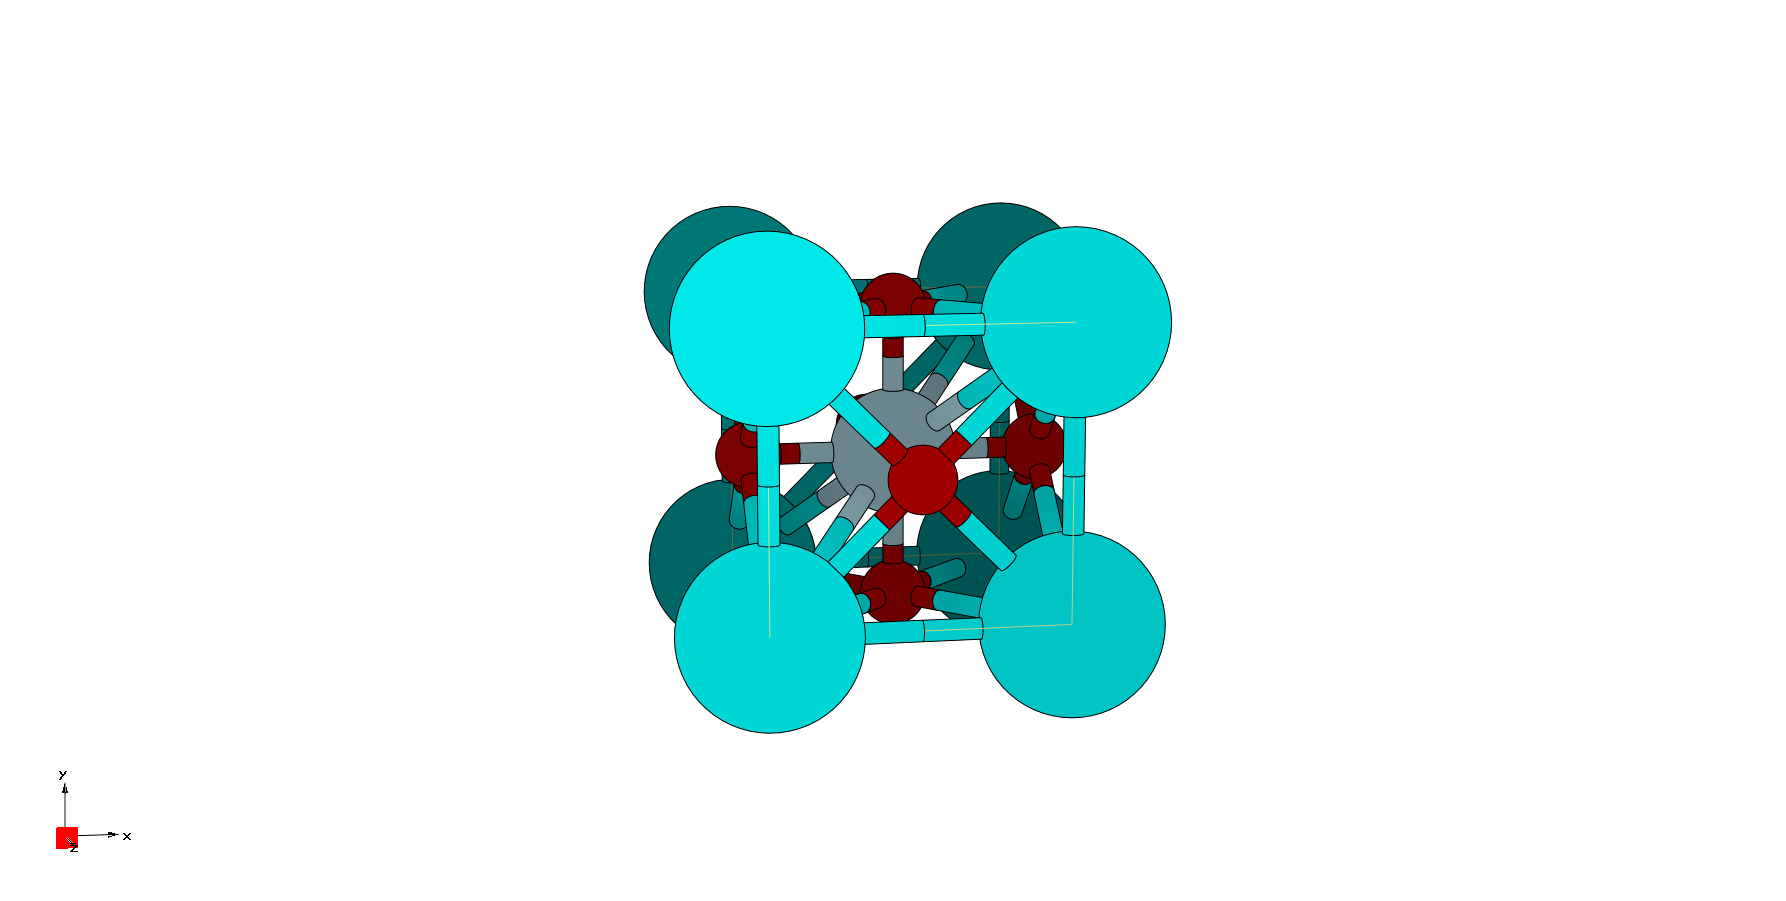
\includegraphics[width=0.45\columnwidth,trim={300pt 10pt 300pt 150pt},clip]{figure/example20/SrMnO3.png}}
\label{fig20}
\caption{Left: atomic structure of epitaxially-strained (tetragonal) LaVO$_3$. Right: atomic structure of epitaxially-strained (tetragonal) SrMnO$_3$. Both structures have been plotted with the \xcrysden{} program.}
\end{figure}
\begin{itemize}
	\item [1-5] These are the usual steps to generate MLWFs and are not reported here.

	\item {\it Inspect the output file {\tt LaVO3.wout}. In the initial summary, you will see that the disentanglement was
performed only within one sphere of radius 0.2 arount the point {\tt A = (0.5, 0.5, 0.5)} in reciprocal space:}

{\small 
\begin{tcolorbox}[sharp corners,boxrule=0.5pt]
\begin{verbatim}
 *------------------------------- DISENTANGLE --------------------------------*
 |  Using band disentanglement                :                 T             |


 	...

 |  Number of spheres in k-space              :                 1             |
 |   center n.   1 :     0.500   0.500   0.500,    radius   =   0.200         |
\end{verbatim}
\end{tcolorbox}
}

\item {\it Compare the band structure that Wannier90 produced with the one obtained using Quantum ESPRESSO.}

To obtain the band structure from the Quantum ESPRESSO calculation we can use the {\tt bands.x} program available at \url{http://www.tcm.phy.cam.ac.uk/~jry20/bands.html}, see minitutorial at the end of Ex.~\ref{sec6:copper}. Here, we only report the {\tt .inp} file used to generate the $k$-point mesh for the non-scf calculation
{\small 
\begin{tcolorbox}[title=bands.x input file LaVO3.inp,sharp corners,boxrule=0.5pt]
\begin{verbatim}
7.03 0.00 0.00
0.00 7.03 0.00
0.00 0.00 7.6627

30

G       0.00000  0.00000  0.00000  M       0.50000  0.50000  0.00000
M       0.50000  0.50000  0.00000  X       0.50000  0.00000  0.00000
X       0.50000  0.00000  0.00000  G       0.00000  0.00000  0.00000
G       0.00000  0.00000  0.00000  Z       0.00000  0.00000  0.50000
Z       0.00000  0.00000  0.50000  A       0.50000  0.50000  0.50000
A       0.50000  0.50000  0.50000  R       0.50000  0.00000  0.50000
R       0.50000  0.00000  0.50000  X       0.50000  0.00000  0.00000
\end{verbatim}
\end{tcolorbox}
}
Remember to add the following line to the {\tt .bands} file in order to show the eigenvalues at each k-point. 
{\tt
\begin{quote}
verbosity      = 'high'
\end{quote}
}
Plot of the interpolated band structure is shown in Fig.~(\ref{fig20.1}). In the top panel, the full band structure is shown. In the bottom panel a magnification around the Fermi energy is shown (similar to Fig. 9 in the Tutorial).
\end{itemize}

\subsection*{Further ideas}
\begin{itemize}
	\item {\it Try to obtain the Wannier functions using the standard disentanglement procedure \dots}

	Plots of the band structure of LaVO$_3$ with full disentanglement and no disentanglement are shown in Fig.~(\ref{fig20.2}). These are plotted against the quantum ESPRESSO band structure (solid black lines) and the Wannier90-interpolated one with disentanglement performed only within a sphere centred in A (red dots). We see that the other two methods diverge from the DFT calculation in region of $k$-space where the bands of interest are not entangled with other unwanted bands. For example, in the zone between $\Gamma$ and M and Z and A the interpolated bands with full disentanglement and no disentanglement diverge substantially from the DFT calculation.  

	\item {\it In order to illustrate all possible cases, it is instructive to apply this method to SrMnO$_3$ \dots}

	Plots of the interpolated bands for the different cases are shown in Fig.~(\ref{fig20.4}). In this case, the disentanglement for all the Mn-3d-derived states (empty red circles in Fig.~(\ref{fig20.4})) is only necessary around the $\Gamma$ point, as for all the other points and lines the bands of interest are well separated from other bands lower in energy. However, if we only consider the $e_g$ states (solid blue circles in Fig.~(\ref{fig20.4})) then the situation is different as these states are entangled with the $t_{2g}$ states around X. Of course the $t_{2g}$ states (solid green cones in Fig.~(\ref{fig20.4})) are entangled with $e_{g}$ states around X and with lower-lying states at $\Gamma$.

\end{itemize}

\begin{figure}[t!]
\centering
\subfloat[Full BS]{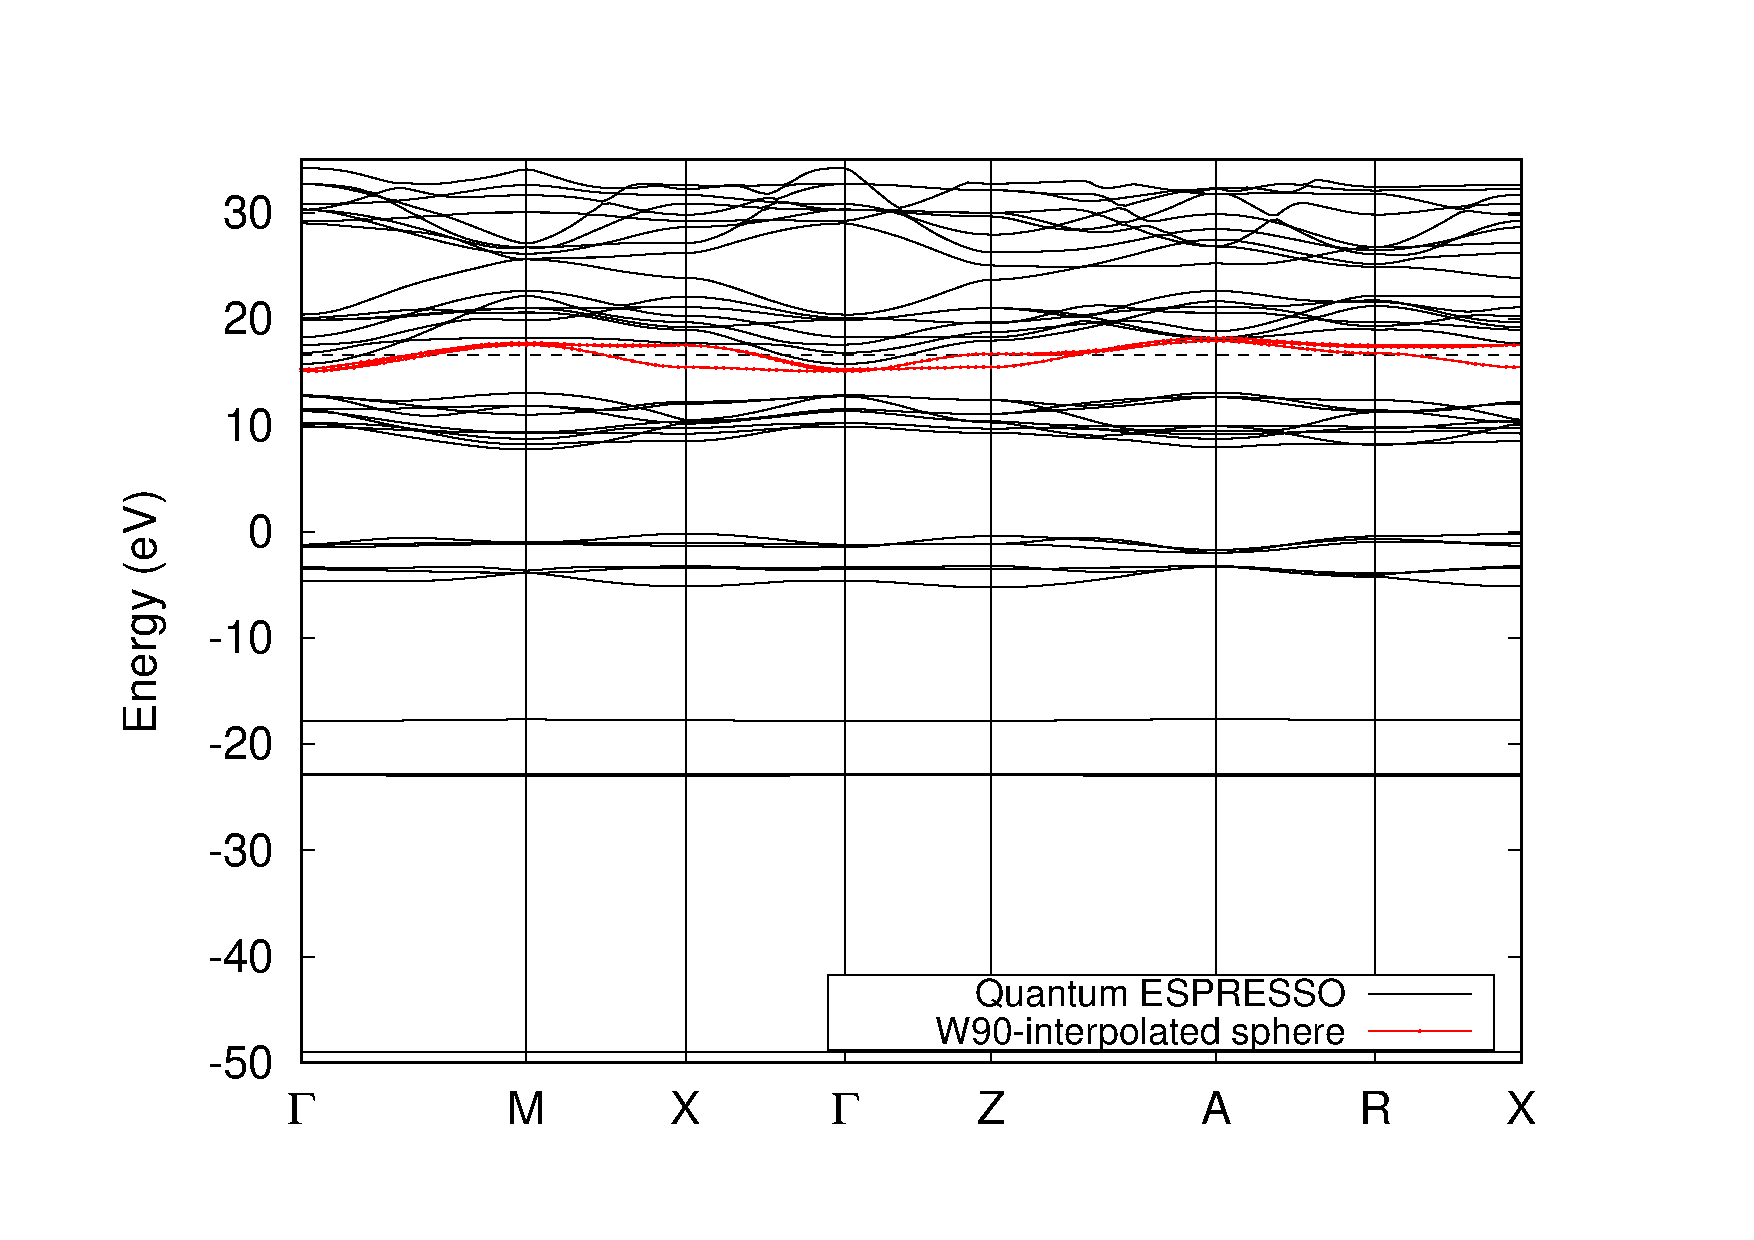
\includegraphics[width=0.7\columnwidth]{figure/example20/LaVO3_full_bandstructure.pdf}}\\
\subfloat[BS around Fermi energy]{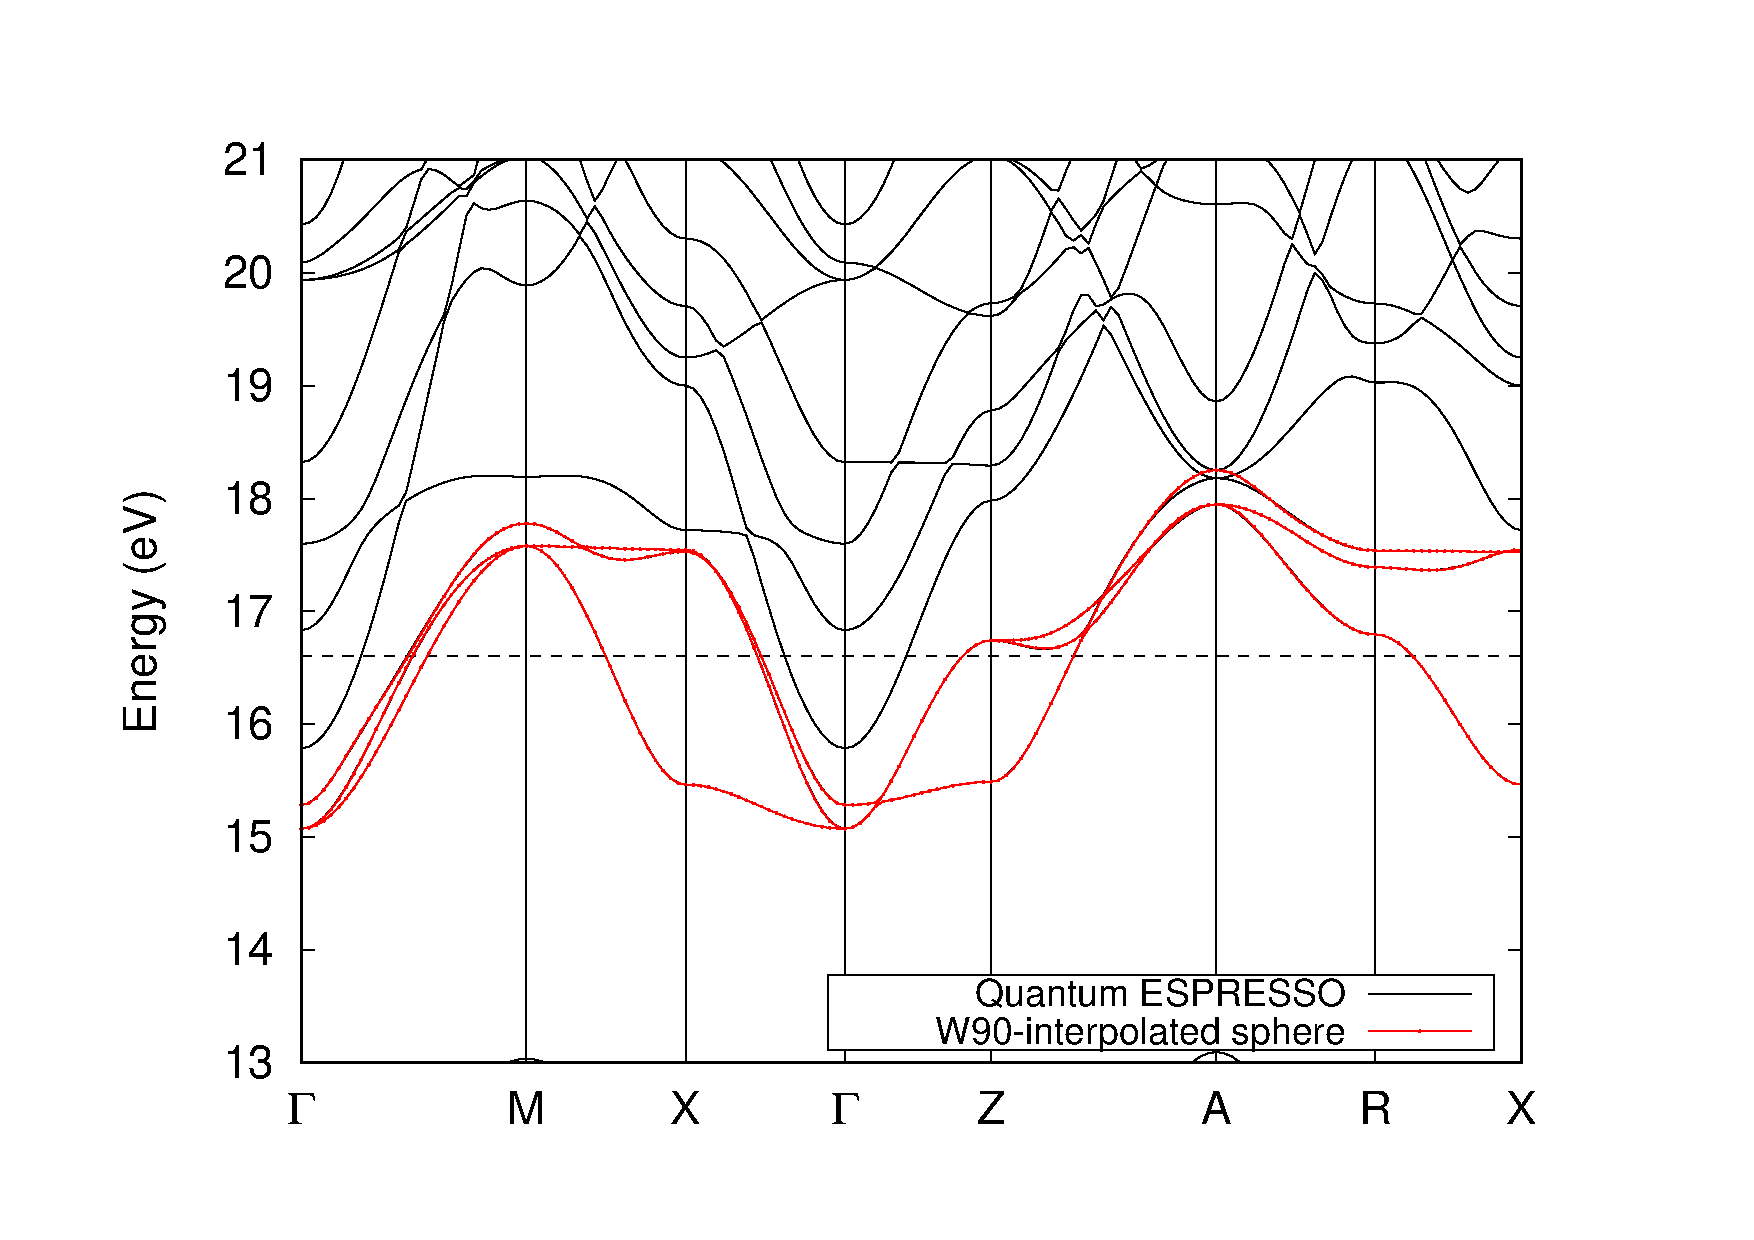
\includegraphics[width=0.7\columnwidth]{figure/example20/LaVO3_bandstructure.pdf}}
\caption{Top panel: full band structure of epitaxially-strained (tetragonal) LaVO$_3$ along the $\Gamma$-M-X-$\Gamma$-Z-A-R-X from DFT calculation (solid black) and interpolation from Wannier90 (red dots). Bottom panel: magnification around Fermi energy $16.6049$ (dashed line). The disentanglement was performed only for $k$-points within a sphere of radius 0.2 $\si{\angstrom}^{-1}$ centered in A.}
\label{fig20.1}
\end{figure}

\begin{figure}[h!]
\centering
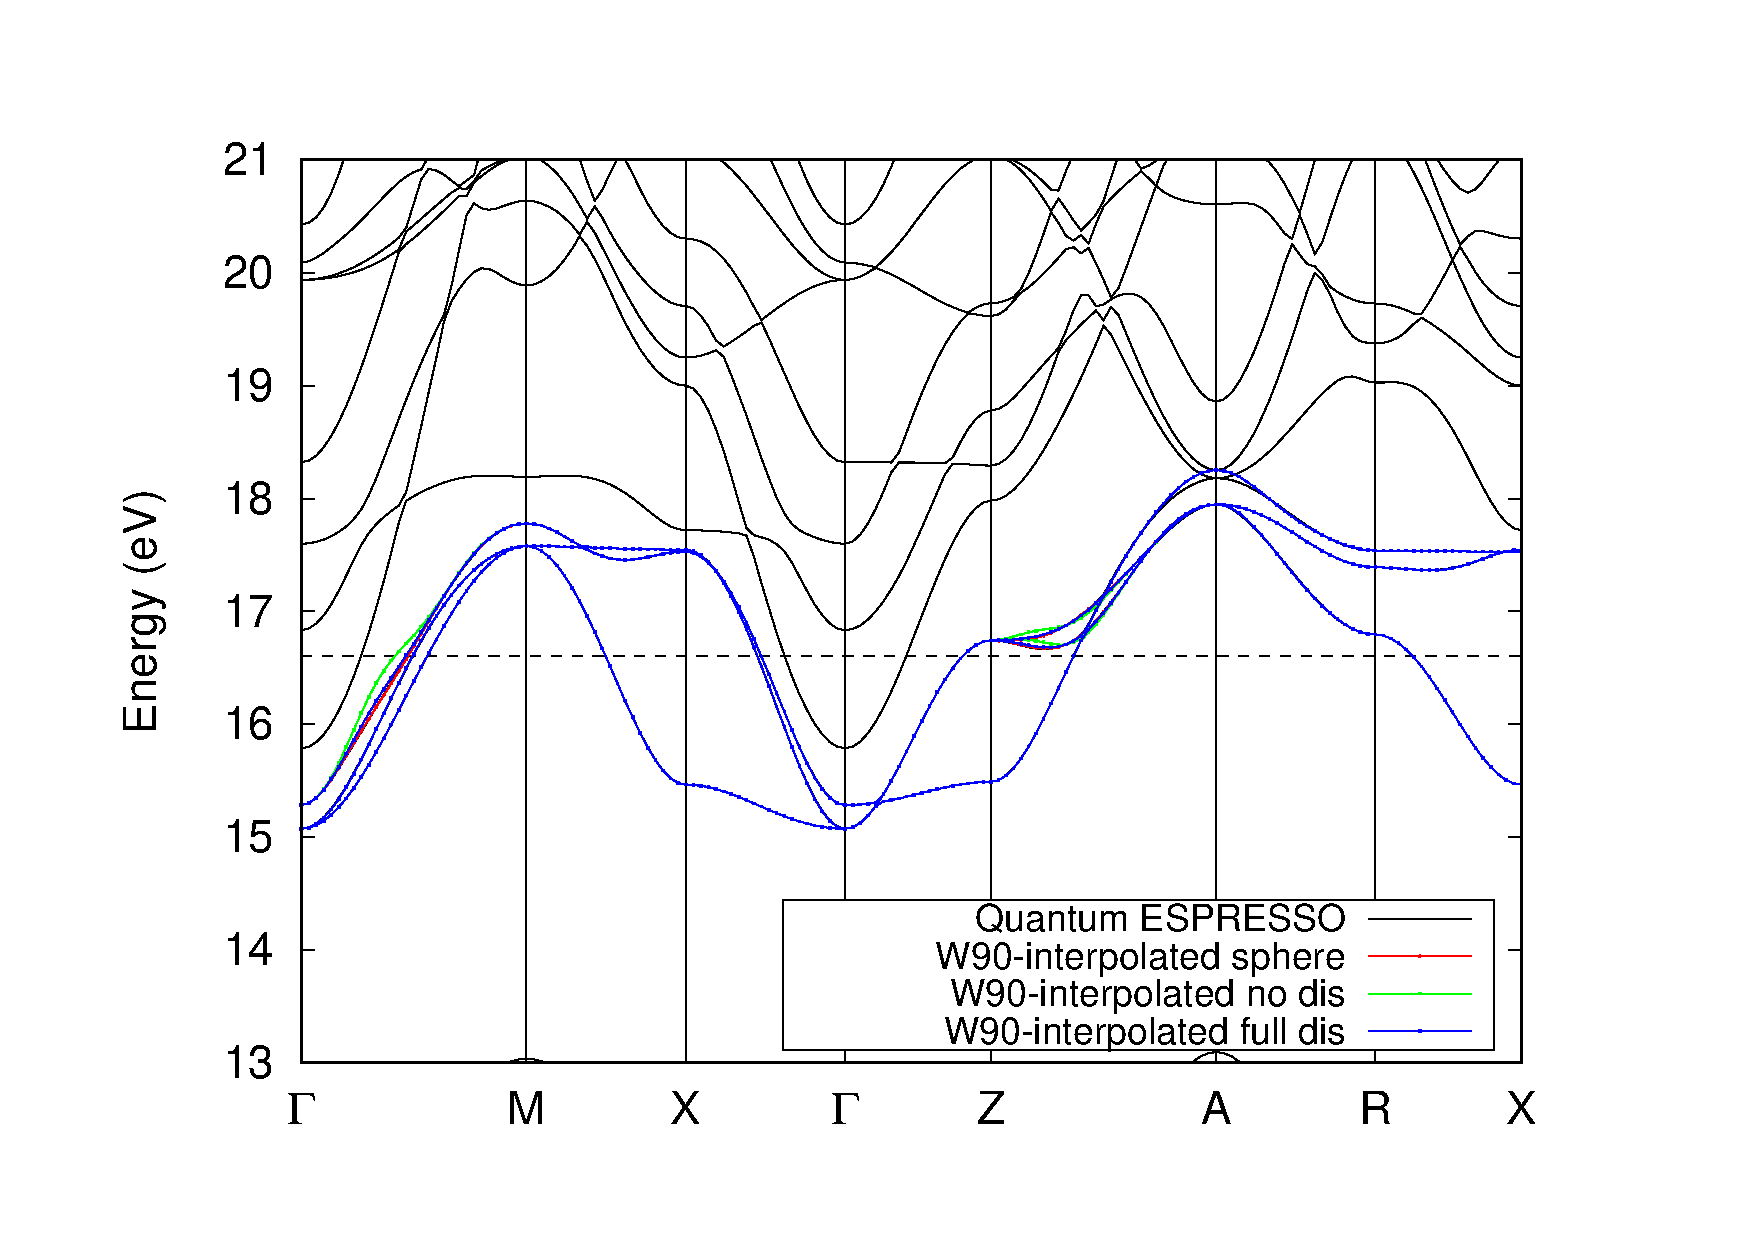
\includegraphics[width=0.7\columnwidth]{figure/example20/LaVO3_bandstructure_all.pdf}
\caption{Comparison of interpolated band structure of epitaxially-strained (tetragonal) LaVO$_3$ with disentanglement on a sphere of radius 0.2 $\si{\angstrom}^{-1}$ centered in A (red dots), full disentanglement (blue dots) and no disentanglement (green dots). Fermy energy is shown with a dashed line.}\label{fig20.2}
\end{figure}

\begin{figure}[h!]
\centering
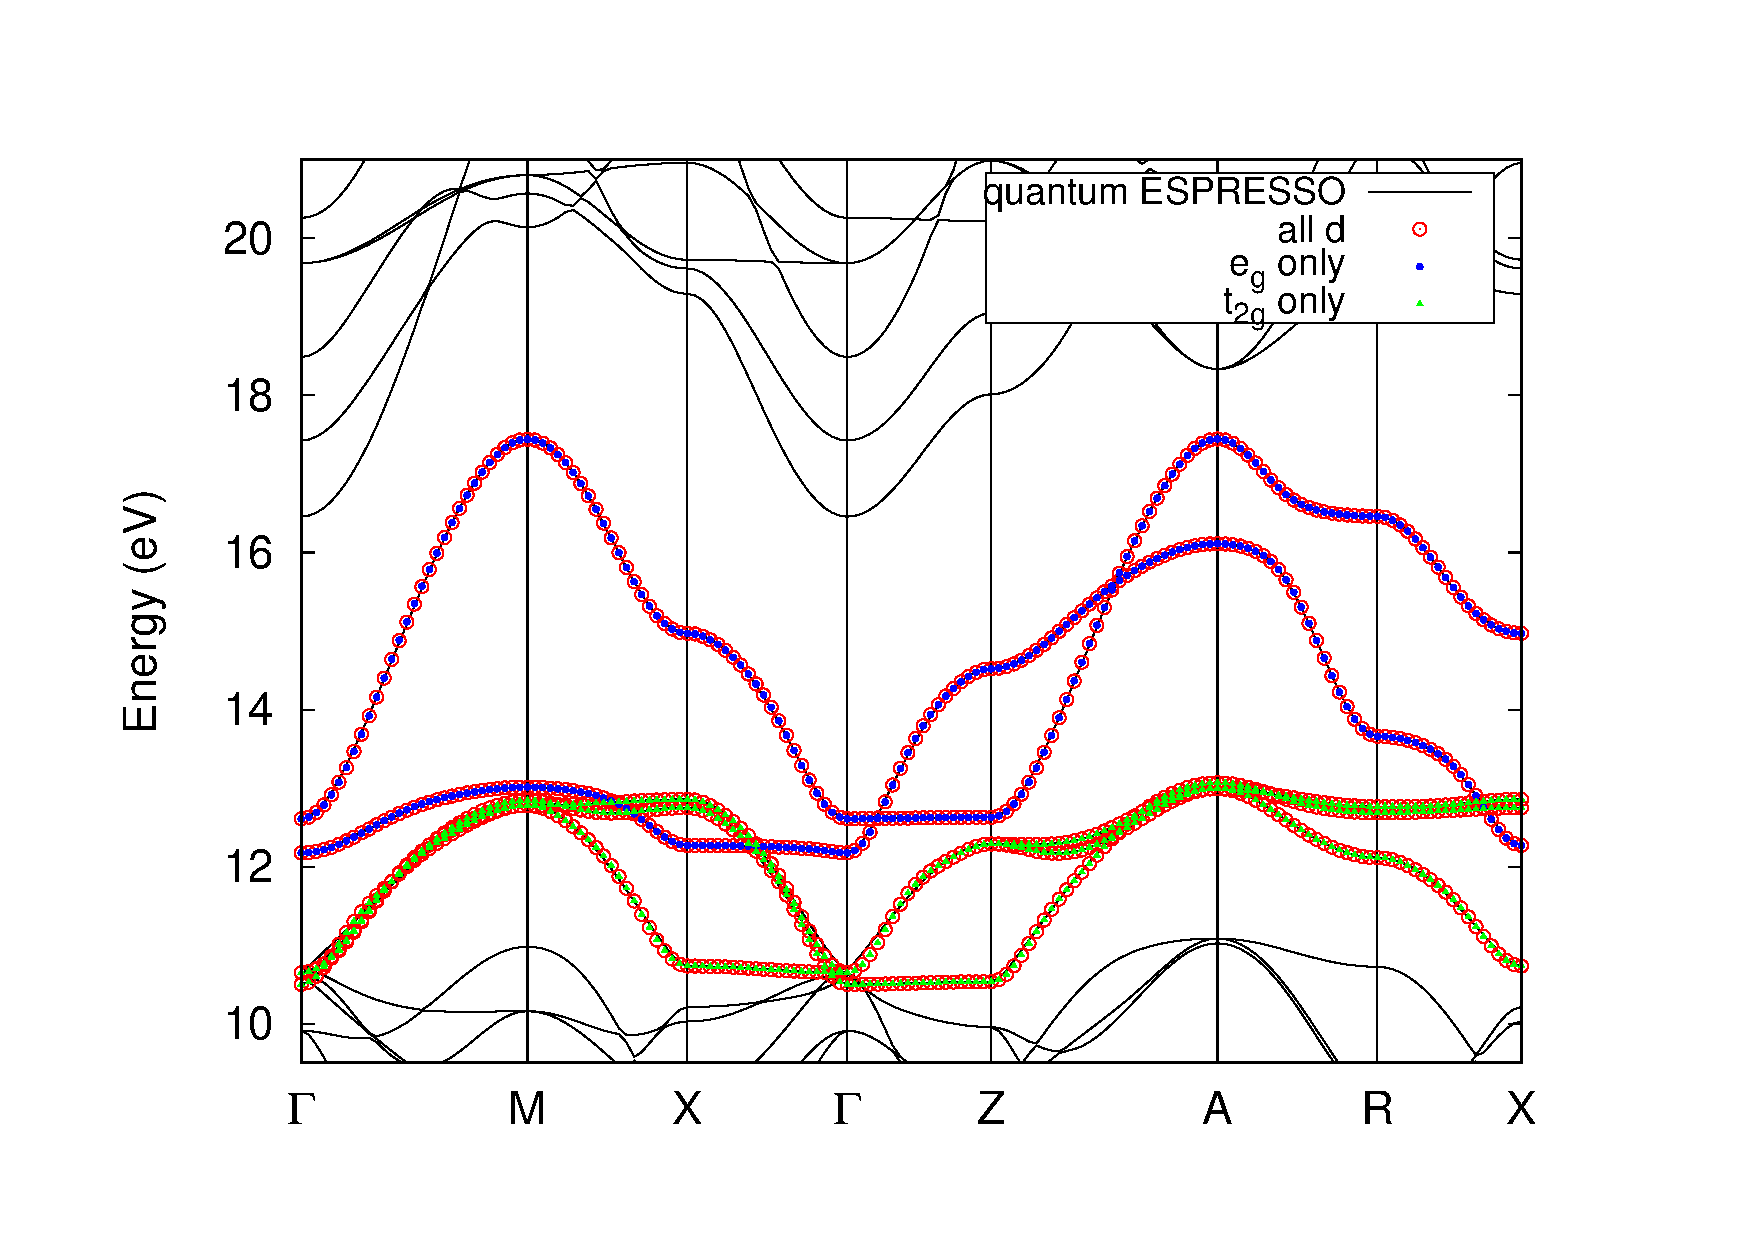
\includegraphics[width=0.7\columnwidth]{figure/example20/SrMnO3_allbands.pdf}
\caption{Wannier90-interpolated bands of SrMnO$_3$. From only $t_{2g}$ states (solid green cones), from only $e_g$ states (solid blue circles), or all Mn-3d-derived states ($t_{2g} + e_g$) (empty red circles).}
\label{fig20.4}
\end{figure}
